% !TEX program = xelatex
\documentclass[a4paper]{article}
\usepackage[a4paper,margin=2.2cm]{geometry}
\usepackage{xeCJK}
\setCJKmainfont{Noto Serif TC}
\setCJKsansfont{Noto Sans TC}
\setmainfont{Times New Roman}
\usepackage{amsmath,amssymb}
\usepackage{graphicx}
\usepackage{booktabs}
\usepackage{caption}
\usepackage[hidelinks]{hyperref}
\usepackage{xurl}
\usepackage{array}
\usepackage{algorithm}
\usepackage{algpseudocode}
\usepackage{enumitem}
\usepackage{xcolor}
\usepackage{tikz}
\usetikzlibrary{shapes.geometric, arrows.meta, positioning, calc}
\usepackage{titlesec}
\titleformat*{\section}{\large\bfseries}
\titleformat*{\subsection}{\normalsize\bfseries}
\setlength{\parindent}{0pt}
\setlength{\parskip}{6pt}
\setlength{\itemsep}{0pt}
\setlength{\tabcolsep}{4pt}
\setlength{\emergencystretch}{3em}
\renewcommand{\baselinestretch}{1.05}
\captionsetup{font=small,skip=4pt}
\setlist[itemize]{leftmargin=1.6em, topsep=2pt, itemsep=2pt, parsep=0pt}
\setlist[enumerate]{leftmargin=1.8em, topsep=2pt, itemsep=2pt, parsep=0pt}
\titleformat{\paragraph}[runin]{\normalfont\bfseries}{}{0pt}{}
\titlespacing*{\paragraph}{0pt}{6pt}{0.6em}

\title{\vspace{-1.2cm}{\fontsize{14}{17}\selectfont\bfseries 114-2 Operations Research Final Project}\\[8pt]
{\fontsize{16}{19}\selectfont\bfseries Optimization-Based Meal Recommendation for Convenience Stores}}
\author{Group 13\;|\;B13705005 宋宇倫、B13705011 陳芃慈、B13705020 陳鼎元、B13705029 蔡冠毅}
\date{}

\begin{document}
\maketitle
\vspace{-0.5cm}

\section{Introduction}
Convenience stores are one of the most frequently used channels for immediate meals among college students and office workers in Taiwan. They are dense, fast to access, and provide relatively complete nutrition labels. However, consumers must often balance multiple factors at once, including price, calories, protein, sugar, sodium, and satiety. A purely price-oriented choice may lead to high-sugar or high-sodium products, while a purely health-oriented choice may make a single meal unnecessarily expensive. In addition, convenience stores frequently offer bundle promotions such as ``rice ball + drink'' or ``noodle dish + egg,'' so the actual payment depends on whether a promotion is activated rather than on a simple sum of listed item prices.

This study formulates the meal selection problem as a mixed-integer linear programming (MILP) model that simultaneously incorporates promotional bundles, personalized nutritional constraints, and historical diversity penalties. After the user specifies a meal scenario (light meal / regular meal / late-night meal), basic physiological information (gender, age, height, and weight), activity level, and health goal (maintenance / fat loss / muscle gain), the model automatically recommends a single-meal combination that satisfies the budget, meets baseline nutritional requirements, and preserves diversity. The central trade-offs of the decision problem include:
\begin{itemize}
\item Cost minimization vs. protein maximization, since high-protein foods are usually more expensive.
\item Strict adherence to nutritional ranges vs. existence of feasible solutions, since overly tight constraints may make the model infeasible.
\item Short-term recommendation diversity vs. repeated selection of objectively ``best'' products.
\end{itemize}
To balance these objectives, the model includes soft penalty terms in the objective function and uses historical weights $h_i$ to control recommendation diversity. Because MILP may require longer solution time when the product set becomes large, this study further proposes a heuristic algorithm, \textbf{GRASP-LS} (Greedy Randomized Adaptive Search Procedure + Local Search), which can return feasible and near-optimal solutions within milliseconds to seconds. Gurobi solutions are used as the benchmark for quantifying the optimality gap.

\section{Problem Description}
Consider a user who is purchasing one meal at a convenience store. Given a set of products, their prices and nutrition labels, and a set of two-item or three-item promotional bundles, the system must determine the following after receiving the user's meal scenario, physiological information, health goal, and budget limit:
\begin{enumerate}
\item which products should be selected as regular-price single items;
\item which promotional bundles should be activated, with all products contained in the activated bundles included in the recommendation;
\item when budget and nutritional conditions conflict, which soft constraints may be moderately relaxed at the minimum penalty cost.
\end{enumerate}

The model outputs a single-meal recommendation list and reports its total calories, protein, fat, carbohydrates, sugar, and sodium. The model must handle both hard constraints---including calorie range, maximum number of items, budget, hard sodium cap, meal-structure requirements, exactly one staple item and at least one protein source for regular meals, and at most one drink and one dessert per meal---and soft constraints, including the protein lower bound, fat and carbohydrate ranges, and sugar and sodium upper bounds. To avoid repeatedly recommending the same products within a short period, the model also applies tiered historical memory penalties to recently recommended products and categories.

\section{Parameter Preprocessing}\label{sec:pre}
User inputs cannot be directly inserted into the MILP. Therefore, this study first converts them into single-meal nutritional parameters using the Mifflin--St Jeor equation. Let age be $A$, height be $H$, weight be $W$, the activity factor be $AF \in \{1.2,1.55,1.725\}$, and the protein factor be $PF \in \{1.1,1.6,1.8\}$. Then
\[
\text{BMR} = \begin{cases}10W+6.25H-5A+5, & \text{male}\\10W+6.25H-5A-161, & \text{female}\end{cases},\quad
\text{TDEE} = \text{BMR}\cdot AF,
\]
\[
\text{Target}_{\text{Cal}} = \text{TDEE} + \delta_{\text{goal}}, \quad
\delta = \{0, -500, +300\} \text{ for \{maintenance, fat loss, muscle gain\}},
\]
\[
\text{Target}_{\text{Pro}} = W \cdot PF, \quad
\text{Target}_{\text{Fat}}^{\min,\max} = \frac{\text{Target}_{\text{Cal}}\cdot FF_{\min,\max}}{9},\quad
\text{Target}_{\text{Carb}}^{\min,\max} = \frac{\text{Target}_{\text{Cal}}\cdot CF_{\min,\max}}{4}.
\]
The daily targets are then scaled down to a single meal using scenario ratios $\rho_m$: $\text{Cal}^{\min,\max}_m = \text{Target}_{\text{Cal}}\cdot \rho^{\min,\max}_m$, and similarly for the other nutrients. This study uses $\rho^{\min,\max}=(0.15,0.25)$ for light meals, $(0.30,0.45)$ for regular meals, and $(0.05,0.15)$ for late-night meals.

\section{Mathematical Model}\label{sec:model}
\paragraph{Sets.}$I$ is the product set, $K$ is the set of promotional bundles, and $S_k\subseteq I$ is the set of products included in bundle $k$. Each product is assigned a meal role according to FamilyMart's official category: $\mathrm{role}(i)\in\{\text{staple},\text{drink},\text{dessert},\text{side}\}$. Let $I^{\mathrm{main}}, I^{\mathrm{drink}}, I^{\mathrm{dess}}\subseteq I$ denote the staple, drink, and dessert sets, respectively. $I^P\subseteq I$ denotes the set of genuine protein sources, defined as products with at least 7 g of protein per serving and not classified as desserts. This prevents high-sugar desserts from being misclassified as protein sources.

\paragraph{Parameters.}$c_i$ is the regular price of product $i$; $cal_i,pro_i,fat_i,carb_i,sug_i,sod_i$ are its nutritional contents; $c_k^{\text{promo}}$ is the promotional price of bundle $k$; $B$ is the budget; $\text{Cal}^{\min,\max}_m, P^{\min}_m,$ \dots are the single-meal requirements defined in \S\ref{sec:pre}; $N^{\max}_m$ is the maximum number of items; $h_i$ is the historical repetition penalty; and $\alpha,\beta,\gamma$ and $\lambda_*$ are objective-function weights.

\paragraph{Decision Variables.}\leavevmode
\[
a_i \in \{0,1\}\ \text{regular single-item selection}, \quad
y_k \in \{0,1\}\ \text{bundle activation}, \quad
x_i = a_i + \sum_{k:\,i\in S_k} y_k \quad\text{(auxiliary variable)}.
\]
Slack variables are $s_P, s^-_{F}, s^+_{F}, s^-_{C}, s^+_{C}, s_{\text{Sug}}, s_{\text{Sod}} \ge 0$.

\paragraph{Tiered Historical Penalty.}To balance short-term non-repetition and the possibility of reintroducing products after sufficient time, this study places recently recommended unique products into a tiered structure inspired by the multi-level feedback queue (MLFQ) in operating systems. Each product is assigned a recency rank $r$ and mapped to a tier $t(r)$. The penalty weight $w(r)=\omega_{t(r)}$ decreases across tiers. We use boundaries $r\le\{3,8,16,30\}$ and weights $\boldsymbol{\omega}=(5,\,2.5,\,1,\,0.3)$. Recently recommended products are placed in the top tier and receive the largest penalty. If they are not selected in subsequent meals, their penalty gradually fades across lower tiers; if they are recommended again, they are promoted back to the top tier. Products are retained up to $r\le 30$, while older records are discarded, which is equivalent to a long but finite memory window. Thus,
\[ h_i = \sum_{r} w(r)\,\mathbf{1}(i\text{ appears in the }r\text{-th most recent record}). \]
In addition, we define a category-level diversity penalty $g_i = \sum_{r} w(r)\,\mathbf{1}\!\big(\mathrm{role}(\text{record}_r)=\mathrm{role}(i)\big)$, which suppresses categories that have just been recommended. This prevents the model from creating only superficial diversity by replacing an item with a same-category variant, such as switching between different brands of soy milk.

\paragraph{Objective.}\leavevmode
\begin{align}
\min\;& \alpha\!\left(\sum_{i\in I} c_i a_i + \sum_{k\in K} c_k^{\text{promo}} y_k\right) - \beta\sum_{i\in I} pro_i x_i + \gamma\sum_{i\in I} h_i x_i + \gamma_{\text{cat}}\sum_{i\in I} g_i x_i \notag\\
& + \lambda_P s_P + \lambda^-_{F} s^-_{F} + \lambda^+_{F} s^+_{F} + \lambda^-_{C} s^-_{C} + \lambda^+_{C} s^+_{C} + \lambda_{\text{Sug}} s_{\text{Sug}} + \lambda_{\text{Sod}} s_{\text{Sod}}. \label{eq:obj}
\end{align}

\paragraph{Constraints.}\leavevmode
\begin{align}
&a_i + \sum_{k:i\in S_k} y_k \le 1, \quad \forall i \in I, \tag{C1: mutual exclusivity}\\
&\sum_{i\in I} c_i a_i + \sum_{k\in K} c_k^{\text{promo}} y_k \le B, \tag{C2: budget}\\
&\text{Cal}^{\min}_m \le \sum_{i\in I} cal_i x_i \le \text{Cal}^{\max}_m, \tag{C3: calorie range, hard}\\
&\sum_{i\in I} pro_i x_i + s_P \ge P^{\min}_m, \tag{C4: protein, soft}\\
&\sum_{i\in I} fat_i x_i + s^-_{F} \ge \text{Fat}^{\min}_m,\quad \sum_{i\in I} fat_i x_i - s^+_{F} \le \text{Fat}^{\max}_m, \tag{C5: fat, soft}\\
&\sum_{i\in I} carb_i x_i + s^-_{C} \ge \text{Carb}^{\min}_m,\quad \sum_{i\in I} carb_i x_i - s^+_{C} \le \text{Carb}^{\max}_m, \tag{C6: carbohydrates, soft}\\
&\sum_{i\in I} sug_i x_i - s_{\text{Sug}} \le \text{Sugar}^{\max}_m, \quad \sum_{i\in I} sod_i x_i - s_{\text{Sod}} \le \text{Sodium}^{\max}_m, \tag{C7--8: sugar/sodium, soft}\\
&\sum_{i\in I} sod_i x_i \le \kappa\cdot \text{Sodium}^{\max}_m, \quad (\kappa = 1.5) \tag{C8b: hard sodium cap}\\
&1 \le \sum_{i\in I} x_i \le N^{\max}_m, \tag{C9: item count}\\
&\sum_{i\in I^{\mathrm{drink}}} x_i \le 1, \quad \sum_{i\in I^{\mathrm{dess}}} x_i \le 1, \tag{C10: meal structure}\\
&\sum_{i\in I^{\mathrm{main}}} x_i = 1, \quad \sum_{i\in I^{P}} x_i \ge 1, \quad \text{if } m = \text{regular meal}. \tag{C11: staple + protein}
\end{align}
Constraint (C8b) is a hard sodium ceiling. Although the soft sodium constraint (C8) allows the sodium level to slightly exceed the target, no meal may exceed $1.5\times$ the sodium limit, thereby preventing overly salty recommendations. Constraint (C10) limits each meal to at most one drink and one dessert. Constraint (C11) requires a regular meal to contain exactly one staple item and at least one genuine protein source, thereby excluding unreasonable combinations such as three snacks as a meal, two drinks as a meal, or a dessert as the main dish.

\paragraph{Interpretation of weights: relative importance of objectives.}The objective-function weights control the relative importance of different objectives: $\alpha$ corresponds to cost, $\beta$ to protein, $\gamma$ and $\gamma_{\text{cat}}$ to repetition penalties, and each $\lambda_*$ to the violation magnitude of a soft constraint. The default setting $(\alpha,\beta)=(1,0.5)$ determines the trade-off scale between cost and protein. The values $\lambda_P=6$, $\lambda_{\text{Sug}}=4$, and $\lambda_{\text{Sod}}=0.15$ determine the penalty intensities for protein deficiency, sugar excess, and sodium excess, respectively. This parameterizes the health--cost trade-off and allows users to directly adjust their preferences through sliders in the app (see the sensitivity analysis in \S\ref{sec:exp}).

\section{Proposed Algorithm: GRASP-LS}\label{sec:alg}
To reduce reliance on commercial solvers in large-scale scenarios, this study designs a heuristic algorithm named \textbf{GRASP-LS}. The method combines greedy randomized construction (GRC) with neighborhood local search (LS), and uses multi-start search to improve global exploration. The overall procedure is shown in Figure \ref{fig:flow} and Algorithm \ref{alg:grasp}.

\paragraph{Core ideas.}
\begin{enumerate}
\item The composite priority score $\sigma(p)$ in Equation \ref{eq:score} jointly evaluates each product's protein contribution, price burden, nutritional fit, category bonus, and historical penalty, giving the greedy construction phase a clear search direction.
\item The RCL (Restricted Candidate List) mechanism uses $\alpha_{\text{rcl}}\in[0.1,0.4]$ to control randomness: $\alpha_{\text{rcl}}\to 0$ approaches a purely greedy search, while $\alpha_{\text{rcl}}\to 1$ approaches a more random search. Each restart samples candidates randomly to generate different initial solutions.
\item Promotional bundles are treated as ``super-items.'' The first step attempts to include one promotional bundle with probability proportional to its score, allowing the heuristic to actively explore the decision boundary between bundle activation and individual-item selection.
\item The construction phase is structure-aware. It first places exactly one staple item and then enforces the at-most-one-drink and at-most-one-dessert constraints while adding later candidates. As a result, the initial solution is structurally feasible and requires less repair by local search.
\item Local search uses multiple moves, including 1-1 swap, 1-0 drop, 0-1 add, and combo-swap. A first-improvement strategy is adopted to accelerate the search and reduce the risk of stagnation.
\item Multi-start search runs GRC+LS over $K_{\text{restart}}=25$ different random seeds, collects all hard-feasible solutions into a solution pool, and returns the solution with the smallest objective value, or a diversified solution sampled from the $\epsilon$-optimal pool described below.
\end{enumerate}
\begin{equation}\label{eq:score}
\sigma(p) = \beta \cdot pro_p - 0.06\alpha\cdot c_p - \gamma h_p - 0.6\tfrac{cal_p}{\text{Cal}^{\max}_m} - \lambda_{\text{Sod}}\tfrac{sod_p}{\text{Sodium}^{\max}_m} - \lambda_{\text{Sug}}\tfrac{sug_p}{\text{Sugar}^{\max}_m} + B_{\text{cat}}(p).
\end{equation}
where $B_{\text{cat}}(p) = 1.2 \cdot \mathbf{1}(p\in I^S) + 1.5\cdot \mathbf{1}(p\in I^P)$.

\begin{figure}[h]
\centering
\scalebox{1.0}{%
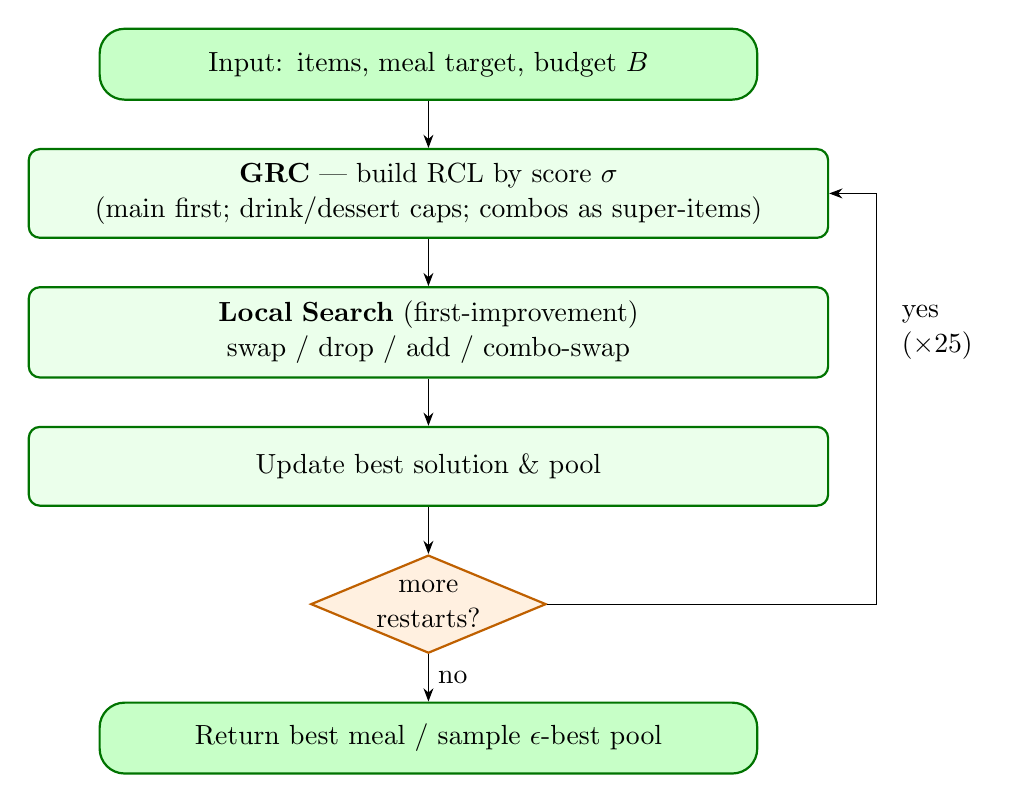
\begin{tikzpicture}[
  font=\normalsize, >=Stealth, node distance=6mm,
  box/.style={rectangle, rounded corners, draw=green!45!black, thick,
              fill=green!8, align=center, inner sep=5pt, text width=98mm, minimum height=10mm},
  term/.style={rectangle, rounded corners=9pt, draw=green!45!black, thick,
               fill=green!22, align=center, inner sep=5pt, text width=80mm, minimum height=9mm},
  dec/.style={diamond, aspect=2.4, draw=orange!75!black, thick, fill=orange!12,
              align=center, inner sep=1pt}]
  \node[term] (in) {Input: items, meal target, budget $B$};
  \node[box, below=of in] (grc) {\textbf{GRC} --- build RCL by score $\sigma$\\(main first; drink/dessert caps; combos as super-items)};
  \node[box, below=of grc] (ls) {\textbf{Local Search} (first-improvement)\\swap / drop / add / combo-swap};
  \node[box, below=of ls] (up) {Update best solution \& pool};
  \node[dec, below=of up] (dec) {more\\restarts?};
  \node[term, below=of dec] (out) {Return best meal / sample $\epsilon$-best pool};
  \draw[->] (in) -- (grc);
  \draw[->] (grc) -- (ls);
  \draw[->] (ls) -- (up);
  \draw[->] (up) -- (dec);
  \draw[->] (dec) -- node[right]{no} (out);
  \draw[->] (dec.east) -| ([xshift=6mm]grc.east) |- (grc.east);
  \node[anchor=west, align=left] at ([xshift=8mm]ls.east) {yes\\($\times25$)};
\end{tikzpicture}}
\caption{Overall GRASP-LS workflow. Under multi-start search, each run constructs a structurally feasible initial solution with GRC, improves it through local search, and updates the solution pool. After $K_{\text{restart}}=25$ restarts, the method returns the best solution. In deployment, it samples from the $\epsilon$-optimal pool to increase diversity and falls back to MILP under extremely tight budgets.}
\label{fig:flow}
\end{figure}

\begin{algorithm}[h]
\caption{GRASP-LS for the Convenience Store Meal Recommendation Problem}
\label{alg:grasp}
\begin{algorithmic}[1]
\Require Instance $\mathcal{I}=(I,K,S)$; single-meal constraints $\mathcal{M}$; weights $w$; budget $B$; number of restarts $K_{\text{restart}}$
\State $s^* \gets \emptyset$; $z^* \gets +\infty$
\For{$r = 1$ \textbf{to} $K_{\text{restart}}$}
  \State $\alpha_{\text{rcl}} \sim \mathcal{U}(0.10, 0.40)$
  \State $s \gets \textsc{GreedyRandomConstruct}(\mathcal{I},\mathcal{M},w,B,\alpha_{\text{rcl}})$
  \Comment{including the ``try bundle first, then add singles'' branch}
  \State $s \gets \textsc{LocalSearch}(s,\mathcal{I},\mathcal{M},w,B)$
  \Comment{1-1 swap / 1-0 drop / 0-1 add / combo-swap, first improvement}
  \State $z \gets \textsc{Evaluate}(s)$
  \If{$s$ is hard-feasible and $z < z^*$} $\;s^* \gets s$; $z^* \gets z$ \EndIf
\EndFor
\State \Return $(s^*, z^*)$
\end{algorithmic}
\end{algorithm}

\paragraph{Time complexity.}At each step, GRC inspects $O(|I|)$ candidates and computes their marginal contributions. It selects at most $N^{\max}_m$ items, so its complexity is $O(N^{\max}_m\cdot |I|)$. In each local-search round, the 1-1 swap neighborhood costs approximately $O(N^{\max}_m\cdot |I|)$. In the worst case, every round improves the solution and triggers another round. In practice, LS converges within $T\le 10$ rounds, giving total runtime $O(K_{\text{restart}}\cdot T\cdot N^{\max}_m\cdot |I|)$.

\begin{algorithm}[h]
\caption{Greedy Randomized Construction (GRC) sub-procedure}
\label{alg:grc}
\begin{algorithmic}[1]
\Require Instance, single-meal constraints, RCL parameter $\alpha_{\text{rcl}}$
\State $s \gets \emptyset$
\If{$\text{Rand}()<0.6$}
    \State Compute $\sigma_k$ for each combo $k$; form an $\alpha_{\text{rcl}}$-RCL from top-scoring combos and randomly select $k^*$ into $s$ \Comment{if $|S_{k^*}|\le N^{\max}_m$}
\EndIf
\While{$|s|<N^{\max}_m$}
    \State Filter uncovered candidates $C$ that do not violate budget or exceed $\text{Cal}^{\max}_m$ after insertion
    \If{$C=\emptyset$} \textbf{break} \EndIf
    \If{$\sum cal_i \ge \text{Cal}^{\min}_m$ and $|s|\ge 2$}
        \State Try the top-3 candidates; add a candidate only if it improves the objective; otherwise \textbf{break}
    \Else
        \State Build an $\alpha_{\text{rcl}}$-RCL by $\sigma$ and randomly add one candidate to $s$
    \EndIf
\EndWhile
\State \Return $s$
\end{algorithmic}
\end{algorithm}

\begin{algorithm}[h]
\caption{Local Search (1-1 swap / 1-0 drop / 0-1 add / combo-swap)}
\label{alg:ls}
\begin{algorithmic}[1]
\Require Solution $s$, maximum number of rounds $T_{\max}$
\For{$t = 1$ \textbf{to} $T_{\max}$}
  \State $\text{improved} \gets \texttt{false}$
  \ForAll{$p \in s$, $p'\notin s$}
    \If{replacing $p$ with $p'$ is feasible and lowers the objective}
      \State $s \gets s\setminus\{p\}\cup\{p'\}$; $\text{improved}\gets\texttt{true}$; \textbf{break to outer}
    \EndIf
  \EndFor
  \If{\textbf{not} improved} Try 1-0 drop, 0-1 add, and combo-swap \EndIf
  \If{no move improves the solution in this round} \textbf{break} \EndIf
\EndFor
\State \Return $s$
\end{algorithmic}
\end{algorithm}

\paragraph{Diversity-aware deployment: $\epsilon$-optimal sampling and fallback solving.}\label{par:eps}
If the system always returns the unique best solution, consecutive queries may produce almost identical meals. MILP is deterministic, and diversity would rely only on historical penalties. This study therefore formalizes diversity as uniform sampling from an $\epsilon$-optimal solution set $\mathcal{S}_\epsilon=\{s : z(s)\le z^*+\epsilon\}$. For each query, the system randomly samples one solution whose objective value is within $\epsilon$ of the best solution. The parameter $\epsilon$ directly controls the trade-off between diversity and optimality, as quantified in \S\ref{sec:div}. In deployment, GRASP-LS with $\epsilon=8$ is used to provide diversified recommendations. If GRASP fails to find a feasible solution under an extremely tight budget, the system falls back to exact MILP solving to ensure that a recommendation is returned whenever a feasible solution exists.

\section{Data Collection and Generation}\label{sec:data}
\paragraph{Real-world data scraping in three stages.}

\textit{Stage 1: nutrition labels.} This study collected official nutrition labels for \textbf{581 real products} from FamilyMart's food-safety traceability API (\url{foodsafety.family.com.tw/Web_FFD_2022/ws/QueryFsProductListByFilter} and \texttt{QueryFsProductByItem}), covering 22 original product categories. Calories, protein, fat, carbohydrates, sugar, and sodium were all obtained from official package-level nutrition labels. The field ``this package contains $n$ servings'' was used to automatically convert serving-level values into package totals. The scraper is implemented in \texttt{src/scrape\_familymart.py}.

\textit{Stage 2: prices.} The food-safety API does not provide prices. We first parsed FamilyMart's fresh-food combo promotion page (\url{nevent.family.com.tw/freshfood/}), which contains six price tiers: \textbf{NT\$49/59/69/79/99/109}. Using n-gram fuzzy string matching, we matched \textbf{124 fresh-food products}, including rice balls, lunch boxes, sandwiches, pasta, and bread, to real in-store prices. For the remaining non-fresh-food items, such as dairy products, beverages, snacks, and frozen foods, FamilyMart does not provide a public single-item in-store price API. Although the FamilyMart e-commerce catalog (\texttt{fts-api.91app.com}) can be scraped, 78\% of its items are box packs or multi-packs, with a median price of NT\$149. These are box-level prices rather than single-item in-store prices. Directly using them would severely distort single-meal pricing, for example by assigning NT\$249 to one bowl of beef noodles. Therefore, the remaining \textbf{457 products} were assigned market-calibrated prices. We established reasonable single-serving price baselines by category, such as about NT\$28 for dairy products, NT\$28 for bottled soy milk, NT\$20 per oden item, and NT\$59 for sous-vide chicken breast, and adjusted beverage prices by volume when capacity information was available. The final price data consist of 124 real fresh-food prices and 457 market-calibrated estimates. The relevant scripts are \texttt{src/scrape\_freshfood\_prices.py} and \texttt{src/curate\_prices.py}. Accordingly, we explicitly label the data sources: fresh foods use real tiered prices, while other products use reasonable market-calibrated estimates.

\textit{Stage 3: serving normalization, family-size filtering, and role labeling.} Many SKUs are multi-serving packages, such as a 1857 ml soy milk bottle with four servings or a 24-piece gift box. Their nutrition and prices describe the entire package rather than the amount appropriate for one meal. We therefore normalized all values to a per-serving basis and imposed a per-serving price floor of NT\$18 to prevent underpriced package averages from generating artificial ``NT\$1 per serving'' products that would dominate the recommendation. Family-size products with at least three servings, such as 1857 ml bottles or 936 ml milk cartons, were removed because they are not realistic single-meal purchases. After filtering, 488 of the 581 products remained. In addition, the original CSV's keyword-based \texttt{is\_main}/\texttt{is\_protein} flags were noisy; cakes and cookies had sometimes been marked as protein sources. We therefore reassigned meal roles using official categories and reclassified sweet breads with sugar $\ge 10$ g, such as pineapple buns and pull-apart buns, as desserts. This makes the definitions of genuine protein source and staple item more consistent with real consumption contexts. The processing logic is implemented in \texttt{src/data\_loader.py}.

\textit{Promotional bundles.} We generated 55 promotional bundles using three rule types: main + drink, main + side, and main + side + drink. The discount rate was set between 17\% and 20\%. This part is a mock setting and is explicitly labeled as such in the report.

\paragraph{Real-world user profiles.}To demonstrate how recommendations differ across user conditions, we designed six representative profiles based on gender, health goal, and activity level. Each profile was paired with three meal scenarios, producing 18 real-world instances (Table \ref{tab:real}).

\paragraph{Random instances.}To evaluate scalability, random instances were generated with product counts $|I|\in\{30,50,80,120,200,300\}$ and bundle counts $|K|\in\{8,15,25,35,60,90\}$. Five random seeds were used for each size, yielding 30 random instances. Product attributes were generated as follows: $cal\sim \mathcal{U}(180,650)$ for staple items or $\mathcal{U}(15,320)$ for non-staples, $pro\sim \mathcal{U}(5,30)$ for protein-containing items or $\mathcal{U}(0,10)$ otherwise, and $sod\sim \mathcal{U}(0,1400)$. Bundle sizes were in $\{2,3\}$, and discount rates were sampled from $\mathcal{U}(0.80,0.92)$ of the original price.

\paragraph{Stress-test scenarios (factorial scenario design).}The random instances above mainly vary the scale factor. To further evaluate the robustness of GRASP-LS under extreme conditions, we designed a $2\times2$ factorial scenario: the first factor is the budget level, tight $B=90$ or loose $B=220$, and the second factor is the protein target, high under the muscle-gain goal or relaxed under the maintenance goal. These factors were crossed with three sizes (80, 120, and 200 products) and four seeds, yielding $4\times3\times4=48$ test instances. Each scenario was solved by both MILP and GRASP-LS using \texttt{src/run\_extra\_experiments.py}. Results are reported in \S\ref{sec:stress}.

\section{Performance Evaluation}\label{sec:exp}
This section compares three solution methods: (i) \textbf{Gurobi MILP}, the exact solver used as the benchmark; (ii) \textbf{GRASP-LS}, the proposed heuristic; and (iii) a \textbf{Greedy baseline}, the simplest protein-to-price-ratio greedy method, used as a very simple heuristic benchmark. The weights are set to $\alpha=1, \beta=0.5, \gamma=2, \gamma_{\text{cat}}=8, \lambda_P=6, \lambda^\pm_F = 2/3, \lambda^\pm_C = 1/1.5, \lambda_{\text{Sug}}=4, \lambda_{\text{Sod}}=0.15$. All MILP/GRASP/Greedy benchmark tables are solved with empty history, so $\gamma$ and $\gamma_{\text{cat}}$ do not affect the optimal values. Diversity effects are evaluated separately in the sensitivity analysis and the ``price of diversity'' experiment.

\subsection{Real-world Instances}
Table \ref{tab:real} reports the results for six real-world users across three scenarios. MILP obtained the global optimum for all 18 instances. GRASP-LS also achieved \textbf{100\% hard-feasibility}, with an average optimality gap of \textbf{7.1\%}; 12 out of 18 instances had zero gap. Importantly, all nonzero gaps occurred in the regular-meal scenario. After the exactly-one-staple and meal-structure constraints (C10--C11) were introduced, the feasible region for regular meals became narrower, and the 1-1 swap neighborhood in GRASP occasionally became trapped in a local optimum, with the worst case being U5 female-maintenance-regular at 40.5\%. By contrast, light meals and late-night meals all had zero gap. The \textbf{Greedy baseline was 0\% feasible under the new structure and hard sodium cap}: it greedily selects small high-protein products according to the protein-to-price ratio, which typically leads to missing a staple item (violating C11) and exceeding the $1.5\times$ sodium cap (violating C8b). This highlights the difficulty of handling multiple structural constraints with a single sorting criterion (Figure \ref{fig:feas}).

\begin{table}[h]
\centering\normalsize
\caption{Complete results for the 18 real-world instances (MILP / GRASP-LS / Greedy). Gap is computed as $(z_{\text{GRASP}}-z_{\text{MILP}})/|z_{\text{MILP}}|$. All MILP runs returned global optima. GRASP-LS was 100\% hard-feasible, with an average gap of 7.1\%; 12 out of 18 gaps were zero, and all nonzero gaps occurred in regular-meal scenarios. Greedy was 0\% feasible due to meal-structure requirements and the hard sodium cap.}
\label{tab:real}
\begin{tabular}{lrrrrrccc}
\toprule
 & & & & & & \multicolumn{3}{c}{Feasible (Y/N)} \\
\cmidrule(lr){7-9}
Instance & Cal range & $P^{\min}$ & MILP obj & GRASP obj & Gap (\%) & MILP & GRASP & Greedy \\
\midrule
U1\_male\_cut-latenight & 106--318 & 11.2 & 27.98 & 27.98 & 0.0 & Y & Y & N \\
U1\_male\_cut-light & 318--529 & 22.4 & 35.80 & 35.80 & 0.0 & Y & Y & N \\
U1\_male\_cut-regular & 635--953 & 44.8 & 87.20 & 119.48 & 37.0 & Y & Y & N \\
U2\_male\_bulk-latenight & 166--497 & 13.5 & 40.60 & 40.60 & 0.0 & Y & Y & N \\
U2\_male\_bulk-light & 497--829 & 27.0 & 68.09 & 68.09 & 0.0 & Y & Y & N \\
U2\_male\_bulk-regular & 994--1491 & 54.0 & 163.53 & 173.55 & 6.1 & Y & Y & N \\
U3\_male\_maintain-latenight & 98--293 & 7.7 & 29.55 & 29.55 & 0.0 & Y & Y & N \\
U3\_male\_maintain-light & 293--489 & 15.4 & 36.21 & 36.21 & 0.0 & Y & Y & N \\
U3\_male\_maintain-regular & 587--880 & 30.8 & 74.04 & 74.85 & 1.1 & Y & Y & N \\
U4\_female\_cut-latenight & 73--220 & 8.3 & 32.91 & 32.91 & 0.0 & Y & Y & N \\
U4\_female\_cut-light & 220--366 & 16.6 & 41.17 & 41.17 & 0.0 & Y & Y & N \\
U4\_female\_cut-regular & 439--658 & 33.3 & 67.74 & 75.05 & 10.8 & Y & Y & N \\
U5\_female\_maint-latenight & 77--232 & 6.1 & 29.62 & 29.62 & 0.0 & Y & Y & N \\
U5\_female\_maint-light & 232--387 & 12.1 & 35.80 & 35.80 & 0.0 & Y & Y & N \\
U5\_female\_maint-regular & 464--697 & 24.2 & 63.20 & 88.82 & 40.5 & Y & Y & N \\
U6\_female\_bulk-latenight & 132--395 & 10.4 & 35.75 & 35.75 & 0.0 & Y & Y & N \\
U6\_female\_bulk-light & 395--659 & 20.9 & 57.55 & 57.55 & 0.0 & Y & Y & N \\
U6\_female\_bulk-regular & 791--1186 & 41.8 & 106.60 & 140.65 & 31.9 & Y & Y & N \\
\bottomrule
\end{tabular}
\end{table}

Figure \ref{fig:break} uses U1 (male, fat loss, regular meal) as an example to compare the nutritional and cost outcomes of the three methods. MILP and GRASP-LS both produce structurally complete meals that satisfy all relevant targets. Greedy, because it only considers the protein-to-price ratio, misses the staple requirement and exceeds the hard sodium cap, making the solution hard-infeasible.

\begin{figure}[h]
\centering
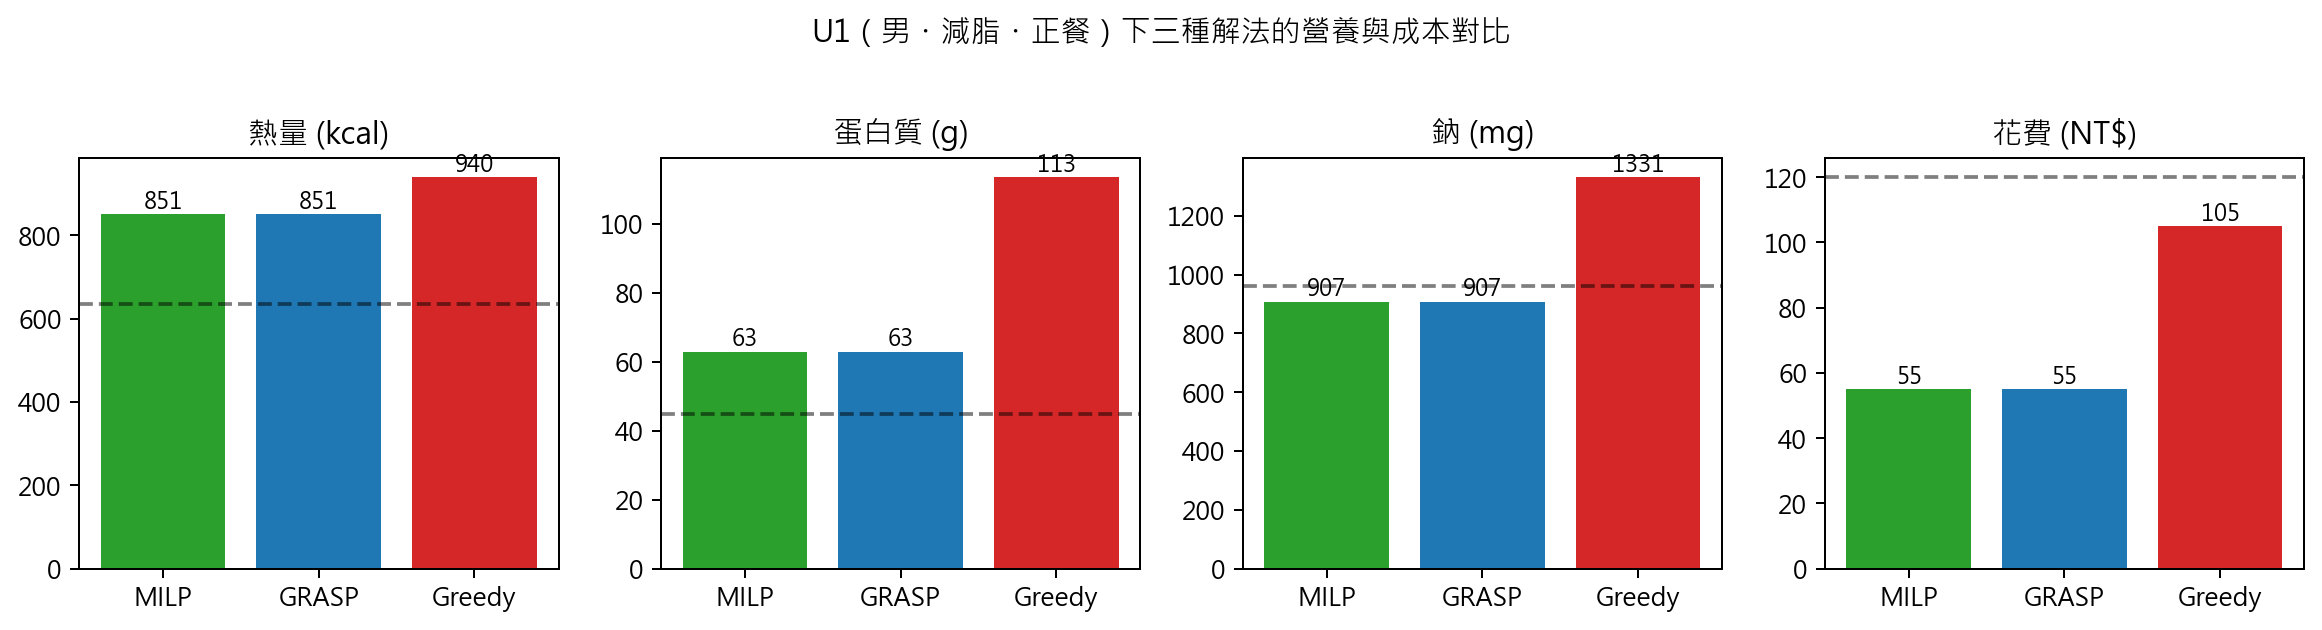
\includegraphics[width=0.95\textwidth]{../results/figs/fig_real_breakdown.png}
\caption{Comparison of calories, protein, sodium, and cost across the three methods for U1 male-fat-loss-regular using 488 real FamilyMart products. Dashed lines indicate the corresponding limits. The MILP solution is a structurally complete meal: pineapple bun (staple) + honey pork jerky (side) + unsweetened thick soy milk (drink) + mixed fruit gummies (dessert), with total cost NT\$110, 693 kcal, 45.6 g protein, and 667 mg sodium. All requirements are satisfied. GRASP-LS selects another near-optimal structured meal (NT\$108). Greedy selects chicken thigh steak + pig-ear strips + soy milk to maximize the protein-to-price ratio, but it lacks a staple item (violating C11) and contains 2168 mg sodium, exceeding the $1.5\times$ hard cap (violating C8b), so it is hard-infeasible.}
\label{fig:break}
\end{figure}

\begin{figure}[h]
\centering
\begin{minipage}{0.46\textwidth}\centering
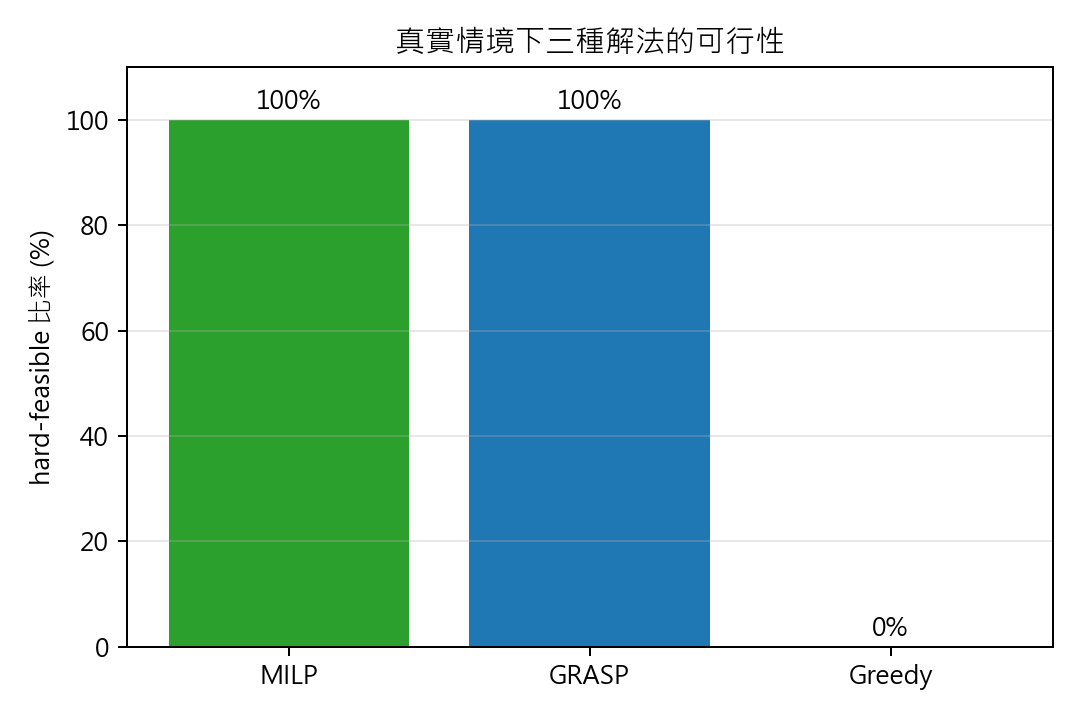
\includegraphics[width=\textwidth]{../results/figs/fig_feasibility.png}
\caption{Hard-feasible rates across the 18 real-world instances.}\label{fig:feas}
\end{minipage}\hfill
\begin{minipage}{0.50\textwidth}\centering
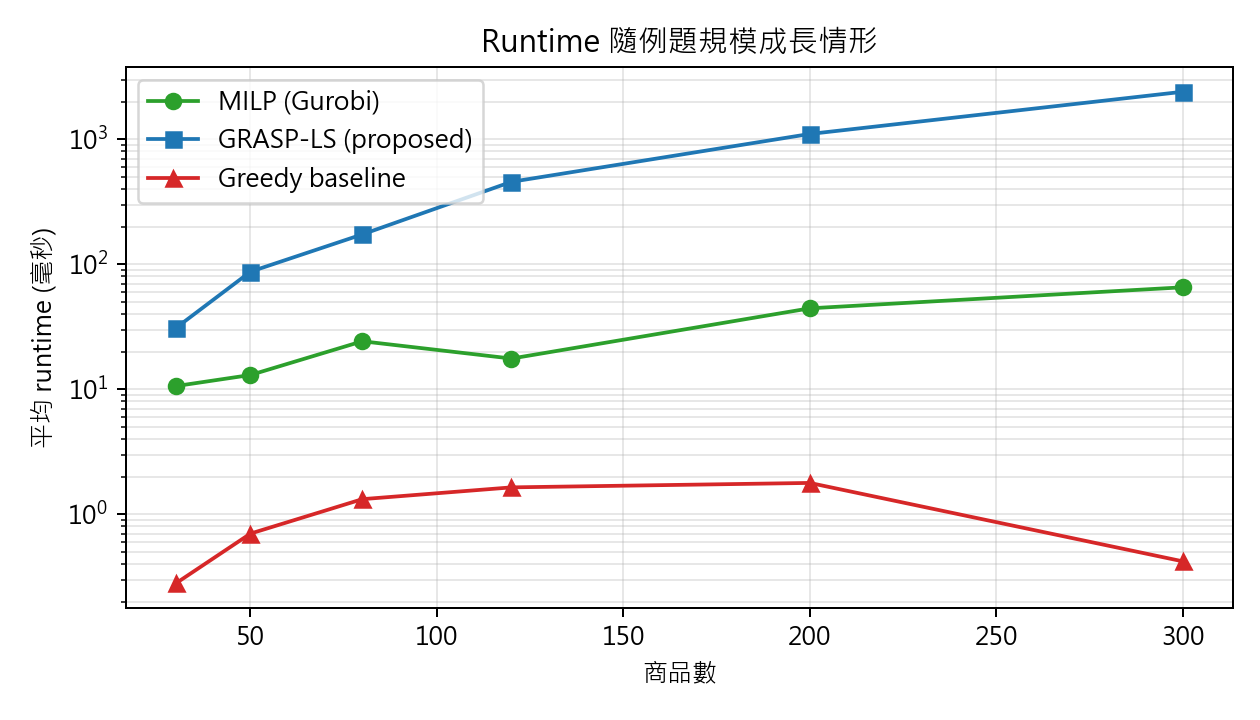
\includegraphics[width=\textwidth]{../results/figs/fig_runtime.png}
\caption{Effect of random-instance size on solution time (log scale).}\label{fig:rt}
\end{minipage}
\end{figure}

\subsection{Random Instances and Scalability}
The results of the 30 random instances are reported in Table \ref{tab:rand} and Figure \ref{fig:gap}.
\begin{table}[h]
\centering\normalsize
\caption{Average performance of the three methods across random-instance sizes, with five seeds per size. Times are in seconds and gaps in percent. The Greedy gap is computed only over its feasible subset; infeasible cases are reflected in the feasibility column.}
\label{tab:rand}
\begin{tabular}{rrrrrrrrr}
\toprule
$|I|$ & $|K|$ & MILP obj & MILP time & GRASP obj & GRASP gap & GRASP time & Greedy feas & Greedy gap \\
\midrule
30 & 8  & 143.5 & 0.006 & 128.6 & -10.3 & 0.017 & 0\% & -- \\
50 & 15 & 111.4 & 0.023 & 94.9  & -14.8 & 0.058 & 20\% & 40 \\
80 & 25 & 74.3  & 0.020 & 74.3  & 0.0   & 0.104 & 0\% & -- \\
120& 35 & 58.6  & 0.075 & 62.4  & 6.5   & 0.576 & 0\% & -- \\
200& 60 & 50.3  & 0.133 & 55.4  & 10.0  & 2.044 & 0\% & -- \\
300& 90 & 42.1  & 0.227 & 44.1  & 4.6   & 4.156 & 0\% & -- \\
\bottomrule
\end{tabular}
\end{table}
MILP found the optimum at every size. GRASP-LS achieved an average optimality gap of \textbf{4.9\%} and a hard-feasible rate of 93\% (28/30). The two cases where GRASP did not find a feasible solution occurred in tight-budget instances with $|I|=30$ and $|I|=50$. Under the structural constraints, greedy construction may occasionally fail to assemble a low-budget meal that contains exactly one staple, at least one protein source, and enough calories. In deployment, these cases are handled by the MILP fallback. It should be noted that the size-level gaps in Table \ref{tab:rand} are averaged over each method's own feasible subset, so the denominators differ. This creates the apparent negative gaps at $|I|=30$ and $|I|=50$ because some seeds are infeasible for GRASP-LS. When computed per aligned instance, the average gap remains \textbf{4.9\%}. By contrast, after adding the meal-structure constraints (C10--C11) and the hard sodium cap (C8b), the Greedy baseline almost completely fails, with \textbf{0\% feasibility} in most sizes. This demonstrates that a single-ratio ranking is insufficient for multi-constraint structured meal selection.
\begin{figure}[h]
\centering
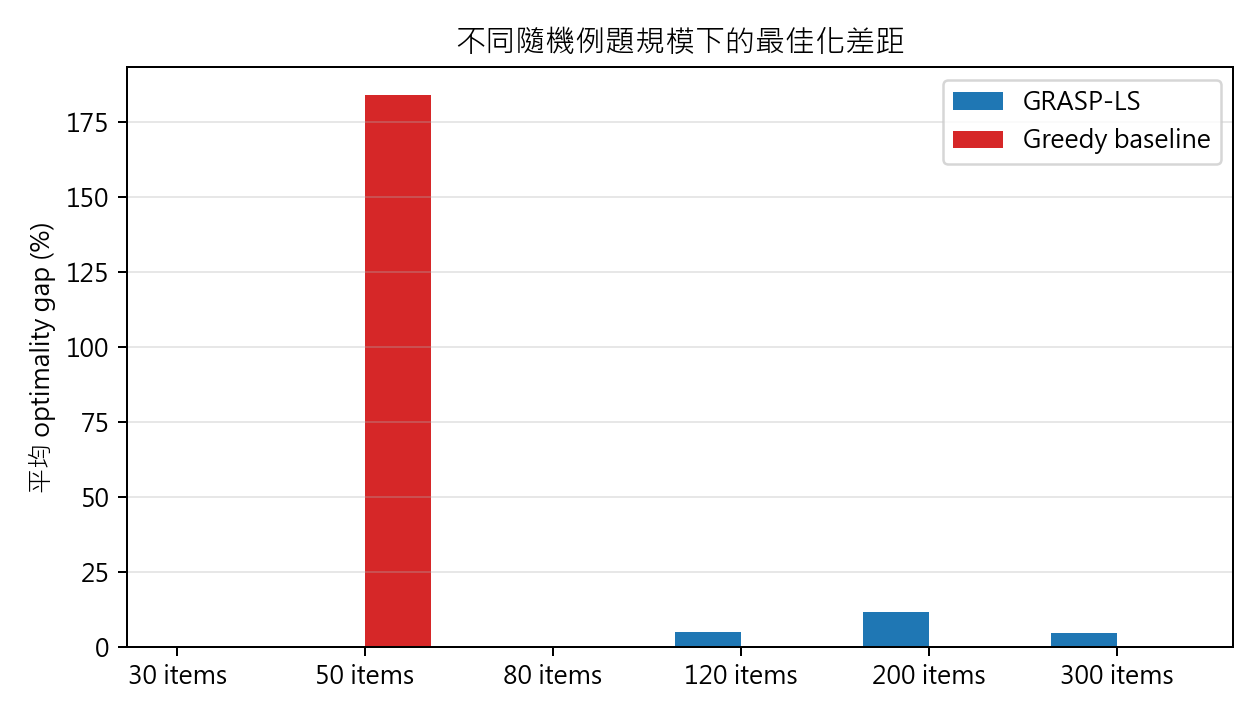
\includegraphics[width=0.7\textwidth]{../results/figs/fig_gap_by_size.png}
\caption{Average optimality gap by random-instance size (GRASP-LS vs. Greedy baseline).}
\label{fig:gap}
\end{figure}

Figure \ref{fig:rt} shows how runtime grows with the number of products. MILP increased from 6 ms at $|I|=30$ to 227 ms at $|I|=300$. GRASP-LS increased from 17 ms to approximately 4.2 seconds. Greedy remained below the millisecond level. Although Gurobi was very fast at the tested scale, GRASP-LS does not require a commercial license, is easier to embed in an app or edge device, and has a controllable anytime property: it can be interrupted at any moment and still return the best solution found so far.

\subsection{Stress-test Scenarios}\label{sec:stress}
Table \ref{tab:stress} summarizes the $2\times2$ stress-test scenarios, where budget and protein target are crossed and each cell contains 12 instances. MILP was feasible in all 48 instances. GRASP-LS found feasible solutions in \textbf{46/48} instances. The two failures both occurred under the tight-budget condition, one with a high protein target and one with a relaxed protein target. The key observation is that \textbf{the high protein target, rather than the tight budget alone, is the main factor that increases the optimality gap}. Under the muscle-gain goal, the gaps were 7.4\% for tight budgets and 4.1\% for loose budgets; under the maintenance goal, the gaps were only 1.2\% and 1.4\%. Tight-budget scenarios were actually faster because the feasible region was smaller (about 1.1--1.2 seconds for GRASP-LS, compared with 2.7--2.9 seconds under loose budgets). Even under the most difficult setting, GRASP-LS maintained an optimality gap no greater than 7.4\% and solved the instances within seconds, confirming its robustness.
\begin{table}[h]
\centering\normalsize
\caption{$2\times2$ stress-test scenarios, with 12 instances per cell: MILP/GRASP-LS feasibility, average GRASP-LS optimality gap, and average solution time.}
\label{tab:stress}
\begin{tabular}{lcccc}
\toprule
Scenario (budget $\times$ protein) & MILP feas & GRASP-LS feas & avg gap & GRASP-LS time \\
\midrule
Tight $\times$ high protein & 12/12 & 11/12 & 7.35\% & 1.10 s \\
Tight $\times$ relaxed      & 12/12 & 11/12 & 1.22\% & 1.24 s \\
Loose $\times$ high protein & 12/12 & 12/12 & 4.12\% & 2.85 s \\
Loose $\times$ relaxed      & 12/12 & 12/12 & 1.36\% & 2.72 s \\
\bottomrule
\end{tabular}
\end{table}

\subsection{Comparison with an Uninformed Shopper}\label{sec:human}
To estimate the model's value relative to the current unaided shopping situation, this study simulates an \textbf{uninformed shopper baseline} over the 488 real products. For each user, 2--4 products were randomly sampled within the user's budget for 4000 trials without any nutritional optimization. The script is \texttt{src/run\_extra\_experiments.py}. The results in Table \ref{tab:human} show that random selection satisfies all single-meal constraints with only about a \textbf{4\%} probability on average. The protein lower bound is satisfied with only about 6\% probability, while the sodium target is satisfied about 63\% of the time. By contrast, GRASP-LS achieves 100\% target satisfaction for all users. Importantly, the model's average spending (about NT\$109) is comparable to the blind-selection average (about NT\$99). The model does \textbf{not} reduce spending by simply buying less. Instead, at nearly the same cost level, it raises the probability of obtaining a fully nutritionally compliant meal from about 4\% to 100\%, while also saving the user the effort of manually calculating nutrition and budget item by item.
\begin{table}[h]
\centering\normalsize
\caption{Uninformed shopper baseline vs. model. Each user is simulated with 4000 random samples. Percentages indicate how often blind selection satisfies each constraint. Model cost is the cost of the GRASP-LS compliant meal.}
\label{tab:human}
\begin{tabular}{lccccc}
\toprule
User & All targets & Protein target & Sodium target & Blind avg. cost & Model cost \\
\midrule
U1 male-fat loss & 5.2\% & 1.6\%  & 59.5\% & NT\$103.7 & NT\$108 \\
U2 male-bulk     & 0.4\% & 1.3\%  & 47.7\% & NT\$121.6 & NT\$149 \\
U3 male-maintain & 3.2\% & 7.1\%  & 71.7\% & NT\$89.5  & NT\$93  \\
U4 female-fat loss & 9.8\% & 5.0\%  & 70.1\% & NT\$89.7  & NT\$94  \\
U5 female-maintain & 3.7\% & 14.6\% & 74.2\% & NT\$80.6  & NT\$85  \\
U6 female-bulk     & 1.9\% & 4.0\%  & 53.2\% & NT\$110.9 & NT\$124 \\
\bottomrule
\end{tabular}
\end{table}

\subsection{Sensitivity Analysis}
Figure \ref{fig:beta} shows the cost-protein trade-off when the budget is relaxed to NT\$220 and the protein weight $\beta$ is varied. When $\beta\le 1$, the model selects an NT\$109.5 combination that just satisfies the protein lower bound (45.6 g). Once $\beta\ge 2$, the marginal benefit of protein exceeds the cost threshold of more expensive high-protein products, so the model changes the recommendation. Protein increases sharply to 92.8 g, and spending rises to NT\$177. At $\beta=8$, the meal reaches 119.5 g of protein and costs NT\$201.5. This stepwise jump reflects the discrete nature of MILP decisions. Figure \ref{fig:gamma} shows the diversity effect of tiered memory. After the optimal solution under $\gamma=0$ is injected into recent history, all four items reappear when $\gamma=0$. Once $\gamma\ge 1$, the tiered penalty causes the model to replace all recommended items, reducing the repetition count to zero. Because the substitutes are similarly inexpensive, total cost even decreases from NT\$109.5 to NT\$103. This indicates that historical penalties can substantially improve diversity with almost no cost sacrifice.
\begin{figure}[h]
\centering
\begin{minipage}{0.48\textwidth}\centering
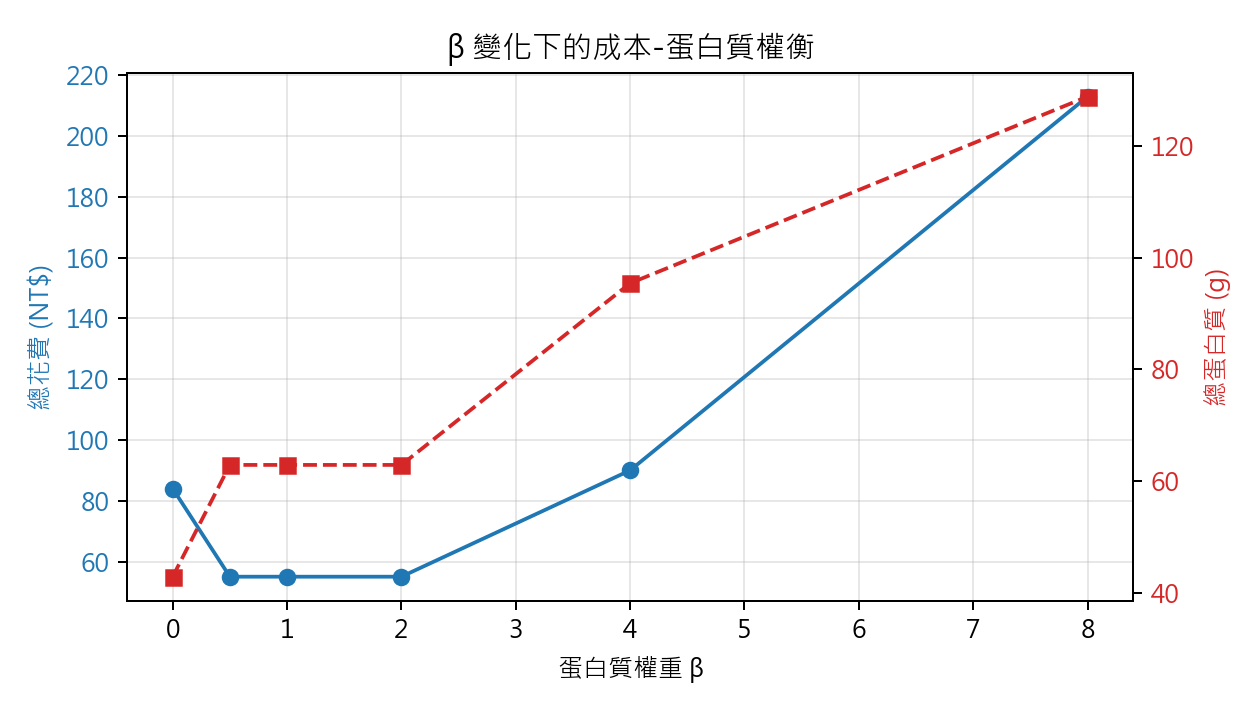
\includegraphics[width=\textwidth]{../results/figs/fig_beta_tradeoff.png}
\caption{Cost-protein trade-off under different values of $\beta$.}\label{fig:beta}
\end{minipage}\hfill
\begin{minipage}{0.48\textwidth}\centering
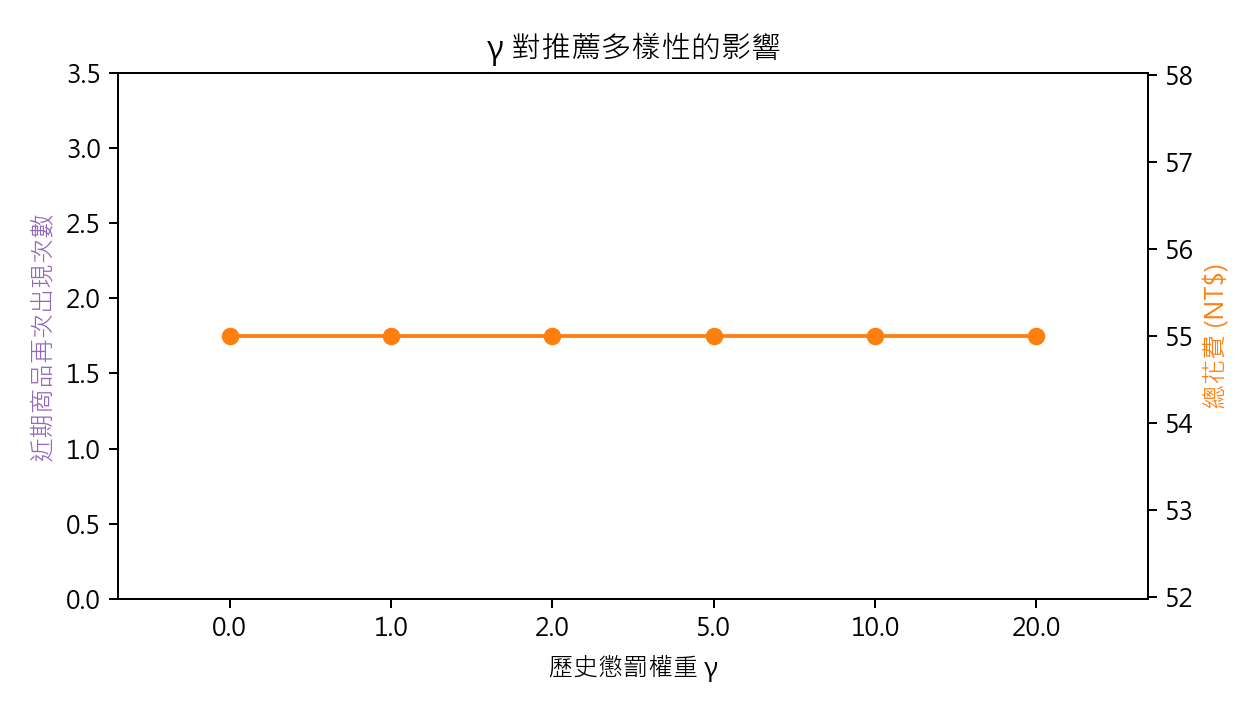
\includegraphics[width=\textwidth]{../results/figs/fig_gamma_diversity.png}
\caption{Decline in recently repeated items as $\gamma$ increases.}\label{fig:gamma}
\end{minipage}
\end{figure}

\subsection{The Price of Diversity}\label{sec:div}
If the system always returns a unique best solution, consecutive queries tend to produce almost the same meal (\S\ref{par:eps}). This study uses the Gurobi solution pool (\texttt{PoolSearchMode=2}) to enumerate the $\epsilon$-optimal solution set $\mathcal{S}_\epsilon=\{s:z(s)\le z^*+\epsilon\}$ and quantify how much optimality must be sacrificed to obtain diversity. For a male-maintenance-regular user whose cheapest compliant meal costs NT\$93, Figure \ref{fig:div} shows that $\epsilon=0$ gives only one optimal meal. Relaxing to $\epsilon=8$ (NT\$8) already provides \textbf{12} structurally complete and distinct meals, with an average additional cost of only NT\$6.7. At $\epsilon=16$, there are \textbf{48} alternatives; at $\epsilon=32$, there are \textbf{641}, with average cost premiums of NT\$12.8 and NT\$20.9, respectively. This curve represents the ``price of diversity'': \textbf{near the optimum, diversity is inexpensive}. By tolerating only a single-digit cost difference, the user can obtain more than ten equally compliant meals. In deployment, this study samples from this set using $\epsilon=8$, approximated by GRASP-LS and combined with tiered long-term memory, to balance optimality and a ``different every time'' user experience.
\begin{figure}[h]
\centering
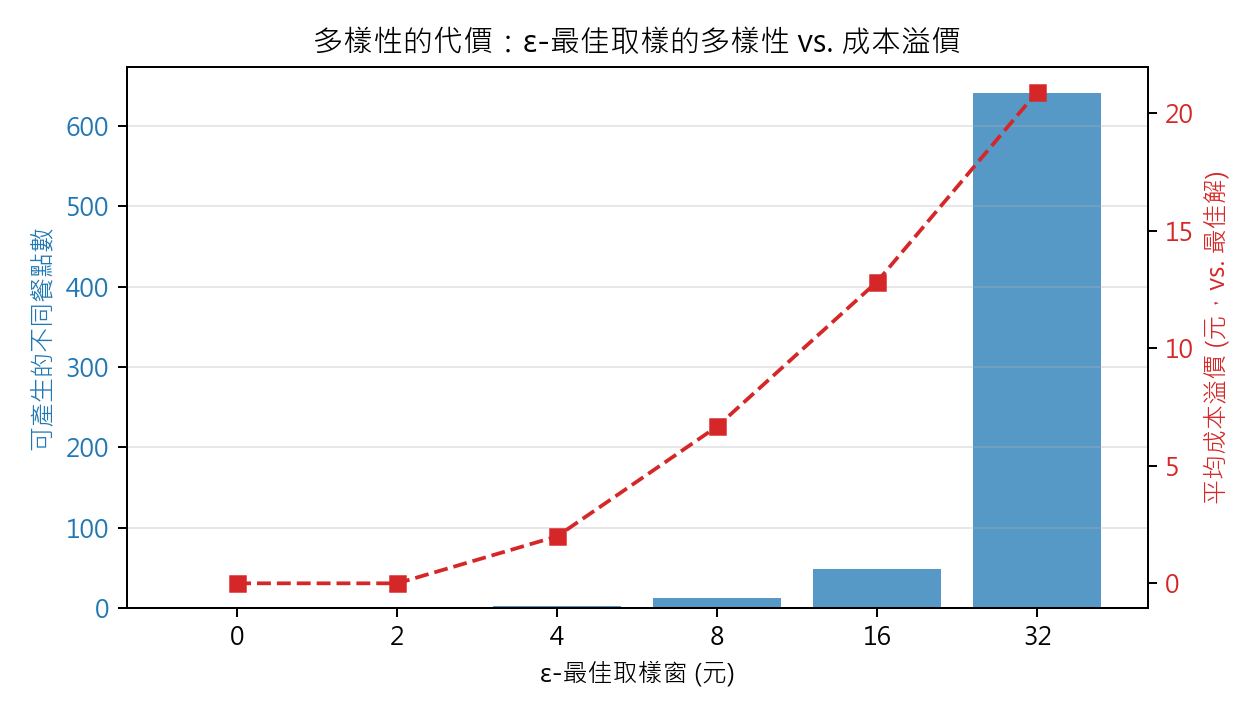
\includegraphics[width=0.62\textwidth]{../results/figs/fig_price_of_diversity.png}
\caption{The price of diversity. As the $\epsilon$-optimal sampling window is relaxed, the number of distinct compliant meals increases from 1 to 641 (blue bars), while the average cost premium (red line) rises only gradually to about NT\$21. Near the optimum, diversity is inexpensive.}
\label{fig:div}
\end{figure}

\subsection{Executable Recommendations}
Consider the U1 male-fat-loss-regular scenario: 70 kg, TDEE 2118 kcal, budget NT\$120, single-meal calorie range 635--953 kcal, protein lower bound 44.8 g, and sodium limit 960 mg. The MILP solution is a structurally complete meal: \textbf{pineapple bun (staple, NT\$24) + honey pork jerky (side, NT\$32) + unsweetened thick soy milk (drink, NT\$28) + mixed fruit gummies (dessert, NT\$25)}. The total cost is NT\$110, with 693 kcal, 45.6 g protein, and 667 mg sodium. It contains exactly one staple item, at least one protein source, one drink, and one dessert, and satisfies the calorie, protein, and sodium targets. By contrast, the Greedy solution based on the protein-to-price ratio selects chicken thigh steak + pig-ear strips + soy milk (NT\$118 and 91 g protein), but it \textbf{lacks a staple item} and reaches 2168 mg sodium, exceeding the $1.5\times$ hard cap. It is therefore not an acceptable recommendation. The value of the model is not merely finding the cheapest meal; a structured meal costs roughly the same as a lunch box. Rather, the model reliably produces meals that are \textbf{structurally reasonable, nutritionally compliant, and different over repeated use} under a fixed budget, which simple price comparison or greedy selection cannot achieve simultaneously.

\subsection{Interactive Web Application}
To validate practical usability, this study implements an interactive Flask web application (\texttt{webapp/app.py}). Users enter physiological information and meal context in the browser. The backend then calls GRASP-LS by default, including $\epsilon$-optimal diversified sampling, or Gurobi MILP, and returns the recommendation list immediately. The web app maintains a tiered ``taste memory'' queue through cookies, allowing users to observe how the MLFQ-style tiered penalty makes consecutive recommendations differ. Users may also adjust $\alpha,\beta,\gamma$ through sliders. A screenshot is shown in Figure \ref{fig:webapp}.
\begin{figure}[h]
\centering
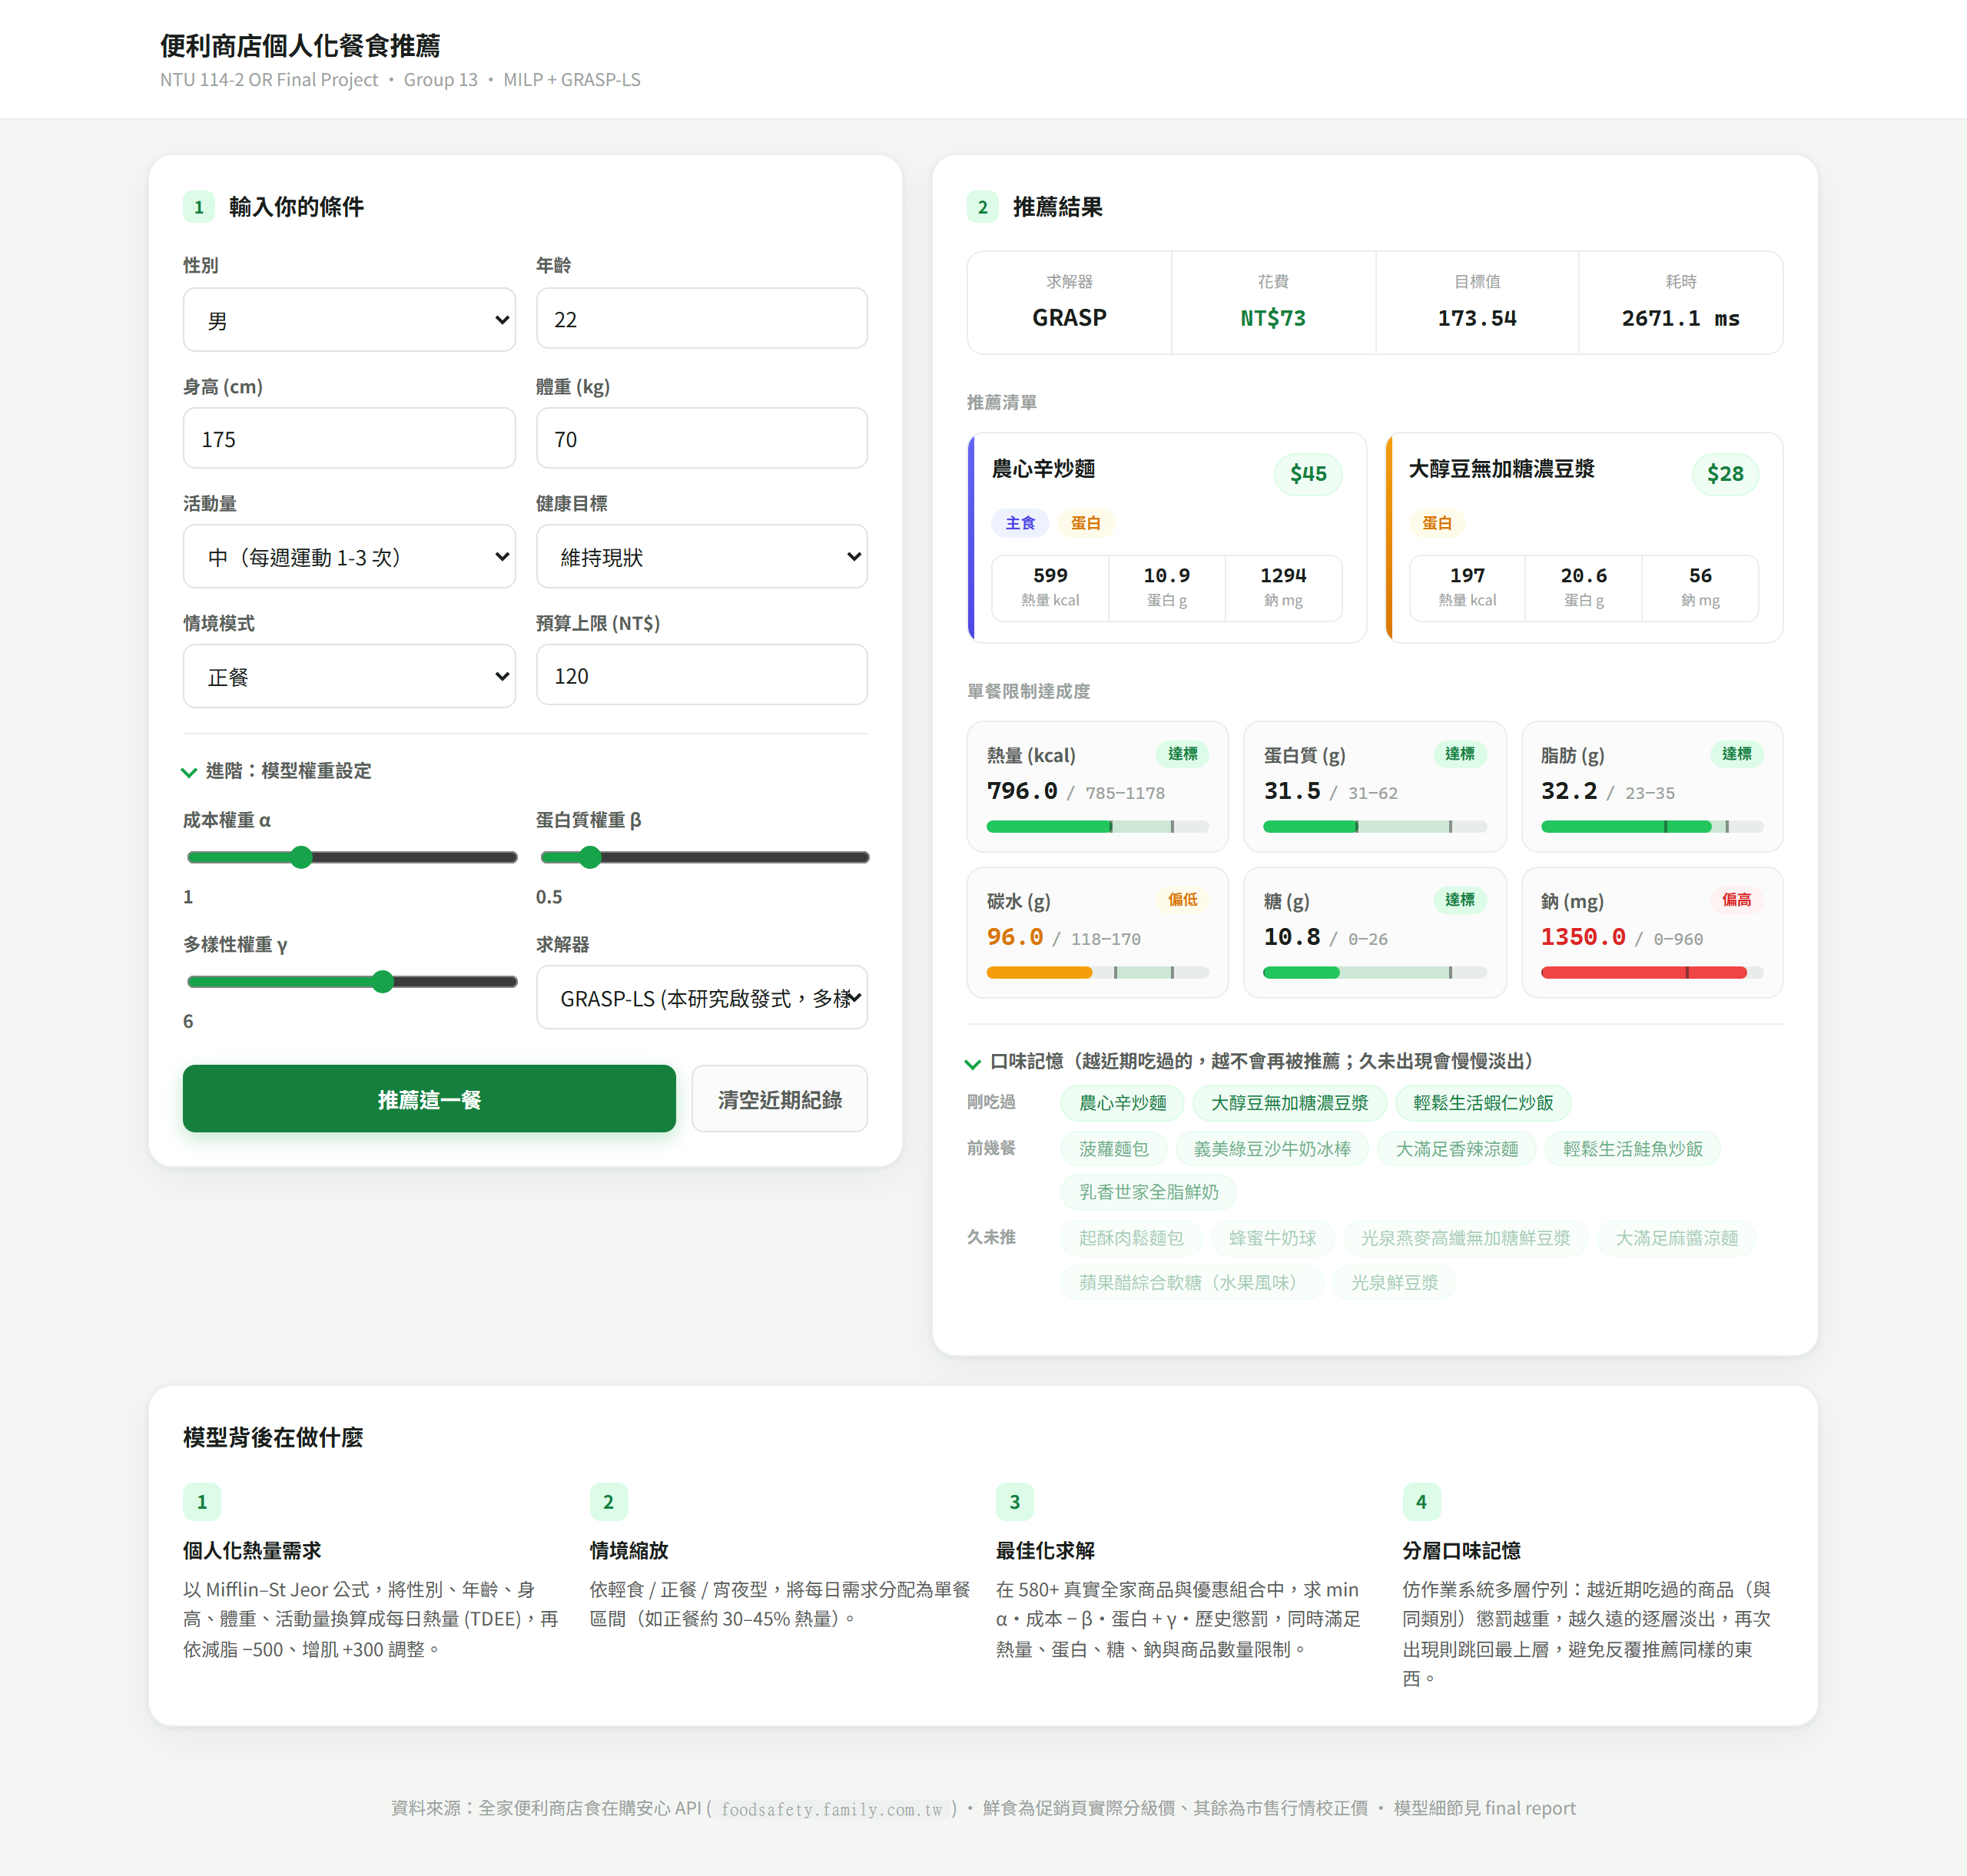
\includegraphics[width=0.95\textwidth]{../results/figs/webapp_result.png}
\caption{Screenshot of the interactive web application, with the advanced weight panel and tiered taste-memory panel expanded. For the input ``male, 22 years old, 175 cm, 70 kg, moderate activity, maintenance, regular meal, budget NT\$120,'' GRASP-LS returns a structurally complete meal and the corresponding nutritional target status. Taste memory is divided by recency into three layers: just eaten, recent meals, and not recommended for a long time. Darker color indicates higher recency and therefore a lower chance of being recommended again. The data come from 488 FamilyMart products; fresh foods use real tiered prices, while other products use market-calibrated estimates.}
\label{fig:webapp}
\end{figure}

\subsection{Discussion and Limitations}
\paragraph{Why is Greedy 0\% feasible under the new model?}Greedy sorts items by a single protein-to-price ratio and adds them sequentially. It therefore tends to select cheap, protein-dense small items such as chicken breast, chicken thigh, and soy milk. As a result, it simultaneously violates multiple hard constraints: it lacks a staple item (C11), consists mostly of side items, and accumulates enough sodium from processed high-protein products to exceed the $1.5\times$ hard sodium cap (C8b). This shows that realistic meal recommendation is a combinatorial optimization problem with multiple structural constraints. No single-ratio ranking can solve it reliably; this is precisely where MILP and GRASP-LS provide value.

\paragraph{Why are GRASP-LS gaps sometimes larger in regular-meal instances?}After the exactly-one-staple and meal-structure constraints (C10--C11) are introduced, the feasible region for regular meals becomes narrower. If the construction phase randomly selects a staple item that is not part of the optimal solution, and the 1-1 swap neighborhood in LS cannot reach the optimal solution in one step, the search may become trapped in a local optimum, with the worst case around 40\%. This can be improved by increasing $K_{\text{restart}}$, adding a dedicated staple-replacement move and 2-2 swap neighborhoods, or falling back to MILP as in the deployment version.

\paragraph{Meal-structure constraints substantially improve recommendation realism.}Earlier versions without C10--C11 and role labels could produce combinations that were numerically nutritionally compliant but unrealistic, such as using a dessert as the main dish, combining three snacks into a meal, or recommending an entire 1857 ml bottle of soy milk. By reassigning roles using official categories, filtering out family-size packages, and adding hard structural constraints requiring exactly one staple and at most one drink and one dessert, the recommendations now resemble realistic meals: one staple item plus a side and/or drink, with at most one dessert. This substantially improves practical adoptability.

\paragraph{Data quality and price estimation.}Nutrition data for the 488 products, after filtering family-size items from the original 581, come from official food traceability records and are therefore highly reliable. For prices, 124 fresh-food items use real tiered prices from the promotion page. The remaining 457 items use category-based market-calibrated prices because FamilyMart provides no public single-item in-store price API and the e-commerce catalog mostly contains box prices, with 78\% multi-pack items. This is the main data limitation of the study. However, sensitivity tests show that when all prices are perturbed by $\pm10\%$, the structure of the U1 regular-meal optimum remains unchanged: staple + side + drink + dessert. The model is therefore robust to small price errors.

\paragraph{Weight selection.}The default weights are $(\alpha, \beta, \gamma)=(1, 0.5, 2)$, and the sensitivity analysis illustrates how these weights affect the solution. In practical deployment, these weights can be exposed through app sliders, allowing users to choose whether they care more about cost or protein. They can also be learned automatically from personal historical feedback.

\section{Conclusions}
This study formulates the convenience-store meal recommendation problem as a mixed-integer linear program that simultaneously incorporates promotional bundles, personalized nutritional constraints, \textbf{meal-structure constraints}, and \textbf{tiered diversity penalties}. The empirical basis is a real dataset of 488 FamilyMart products, where fresh foods use real tiered prices and other items use market-calibrated price estimates. To balance solution quality and practical usability, this study develops a GRASP-LS heuristic with structure-aware construction and $\epsilon$-optimal diversified sampling, and evaluates it on 18 real-world and 30 random instances. The main findings are as follows. (1) MILP obtains global optima within milliseconds to seconds. (2) GRASP-LS achieves 100\% hard-feasibility in real-world instances, with average optimality gaps of 7.1\% for real-world instances and 4.9\% for random instances. (3) After adding meal-structure constraints and the hard sodium cap, the simplest Greedy method becomes \textbf{0\% feasible}, highlighting the necessity of combinatorial optimization under multiple structural constraints. (4) Sensitivity analysis shows that $\beta$ controls the cost-protein trade-off in a stepwise manner, while tiered historical penalties can eliminate repetition with almost no price increase. (5) The Gurobi solution pool quantifies the \textbf{price of diversity}: near the optimum, allowing an NT\$8 window yields 12 compliant meals, and an NT\$32 window yields 641, indicating that diversity is inexpensive near the optimal solution. (6) The implemented Flask web application, with tiered taste memory and weight sliders, demonstrates the model's deployment potential.

Future work can extend the framework in several directions: (a) multi-day sequential recommendation and dynamic inventory or arrival information; (b) integration with in-store OCR-based product-label recognition to update the dataset automatically; (c) online learning from user clicks and rejections, so that $h_i$ reflects not only past recommendations but also learned preferences; and (d) integration with delivery apps to expand the recommendation scope to multiple channels, such as 7-11 and Hi-Life, as well as time-limited products.

\end{document}
